
\begin{frame}{My Contribution towards issues/challenges}
    \begin{figure}
        \centering
        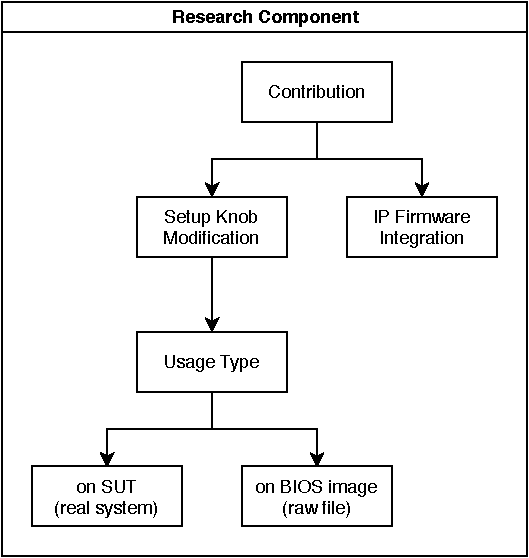
\includegraphics[width=0.6\linewidth]{Im/figures/research-component.pdf}
        % \caption{Research Component}
%        \label{fig:research-component}
    \end{figure}
\end{frame}

\begin{frame}[allowframebreaks]{Setup Knobs Modification: Process Flow}
    \begin{figure}[htbp]
        \centering
        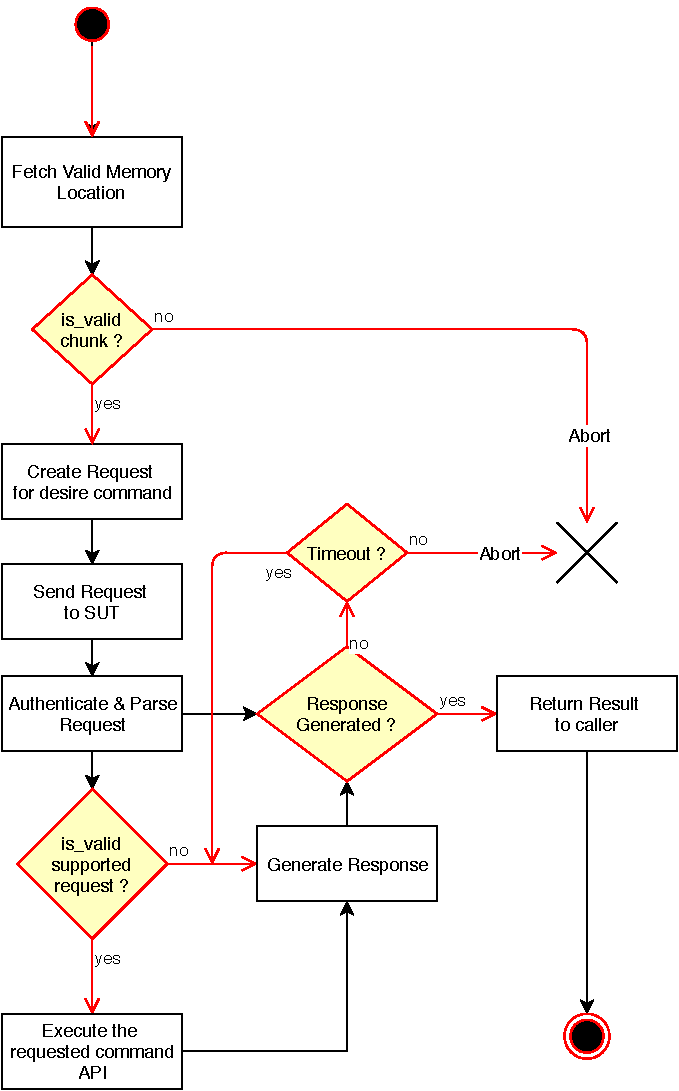
\includegraphics[width=0.3\linewidth]{Im/figures/mod-setup-knobs-flow.pdf}
        \caption{Setup Knobs Modification Flow on SUT}
        \label{fig:setup-knobs-flow}
    \end{figure}
    
%    \begin{figure}[htbp]
%        \centering
%        \includegraphics[width=0.3\linewidth]{Im/figures/setup-knobs-flow-bios.pdf}
%        \caption{Setup Knobs Modification Flow on BIOS image}
%        \label{fig:setup-knobs-flow-bios}
%    \end{figure}
\end{frame}


\begin{frame}[allowframebreaks]{Setup Knobs Modification: Implementation Snaps}
    
    \begin{figure}[htbp]
        \centering
        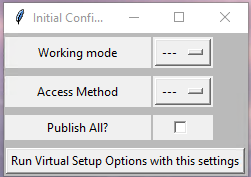
\includegraphics[width=0.6\linewidth]{Im/figures/proposed-work/bios-gui-initial-config}
        \caption{Menu to Select initial configuration for work}\label{fig:proposed-work-bios-gui-initial-config}
    \end{figure}
    
    \begin{figure}[htbp]
        \centering
        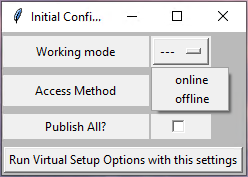
\includegraphics[width=0.6\linewidth]{Im/figures/proposed-work/bios-gui-initial-config-select-mode}
        \caption{Available work mode for the system: Online and Offline}\label{fig:proposed-work-bios-gui-initial-config-select-mode}
    \end{figure}

    \begin{figure}[htbp]
        \centering
        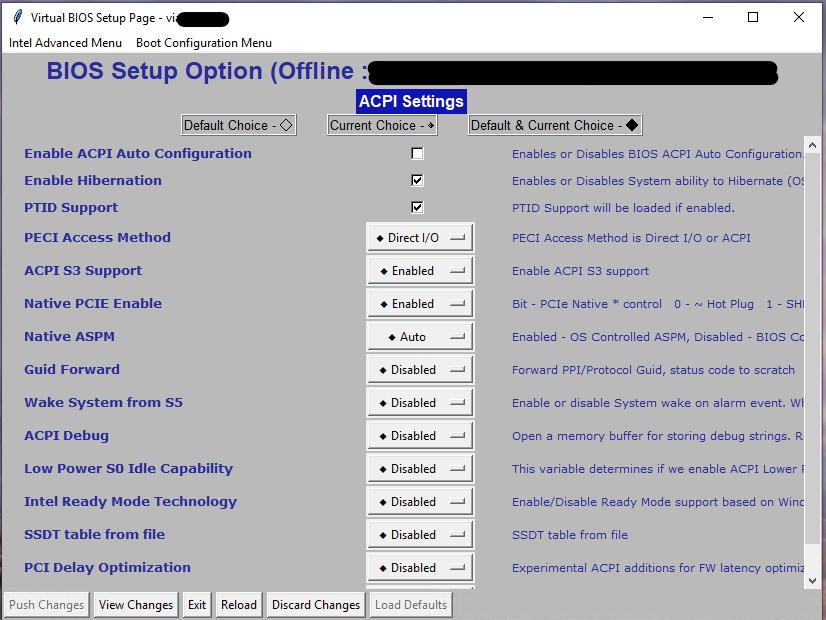
\includegraphics[width=0.6\linewidth]{Im/figures/proposed-work/bios-gui-acpi-knobs}
        \caption{Setup Options listed under ACPI Configurations}\label{fig:proposed-work-bios-gui-acpi-knobs}
    \end{figure}

    \begin{figure}[htbp]
        \centering
        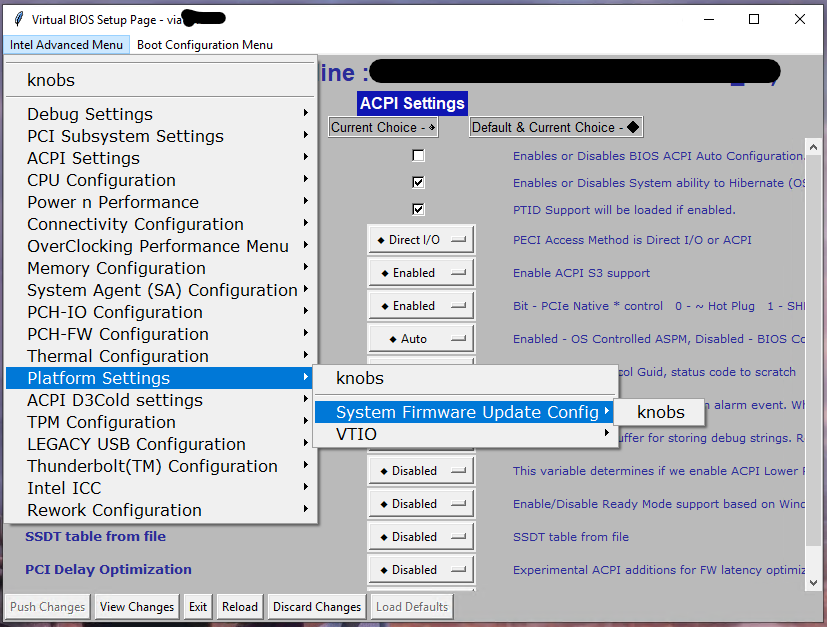
\includegraphics[width=0.6\linewidth]{Im/figures/proposed-work/bios-gui-accessing-menu}
        \caption{Navigating through BIOS setup page}\label{fig:proposed-work-bios-gui-accessing-menu}
    \end{figure}
\end{frame}

\begin{frame}{Setup Knobs Modification: Outcome}
    \begin{itemize}
        \item Cross platform usage
        \item API as a driver in BIOS Firmware
        \item Generic solution for usage types - on \textbf{SUT}, on \textbf{BIOS image}
        \item Information parsing and simulation
        \item Realtime sync for simulation changes
        \item Seamless Integration
    \end{itemize}
\end{frame}


\begin{frame}{IP firmware Integration: Structure of Module}
    \begin{figure}[htbp]
        \centering
        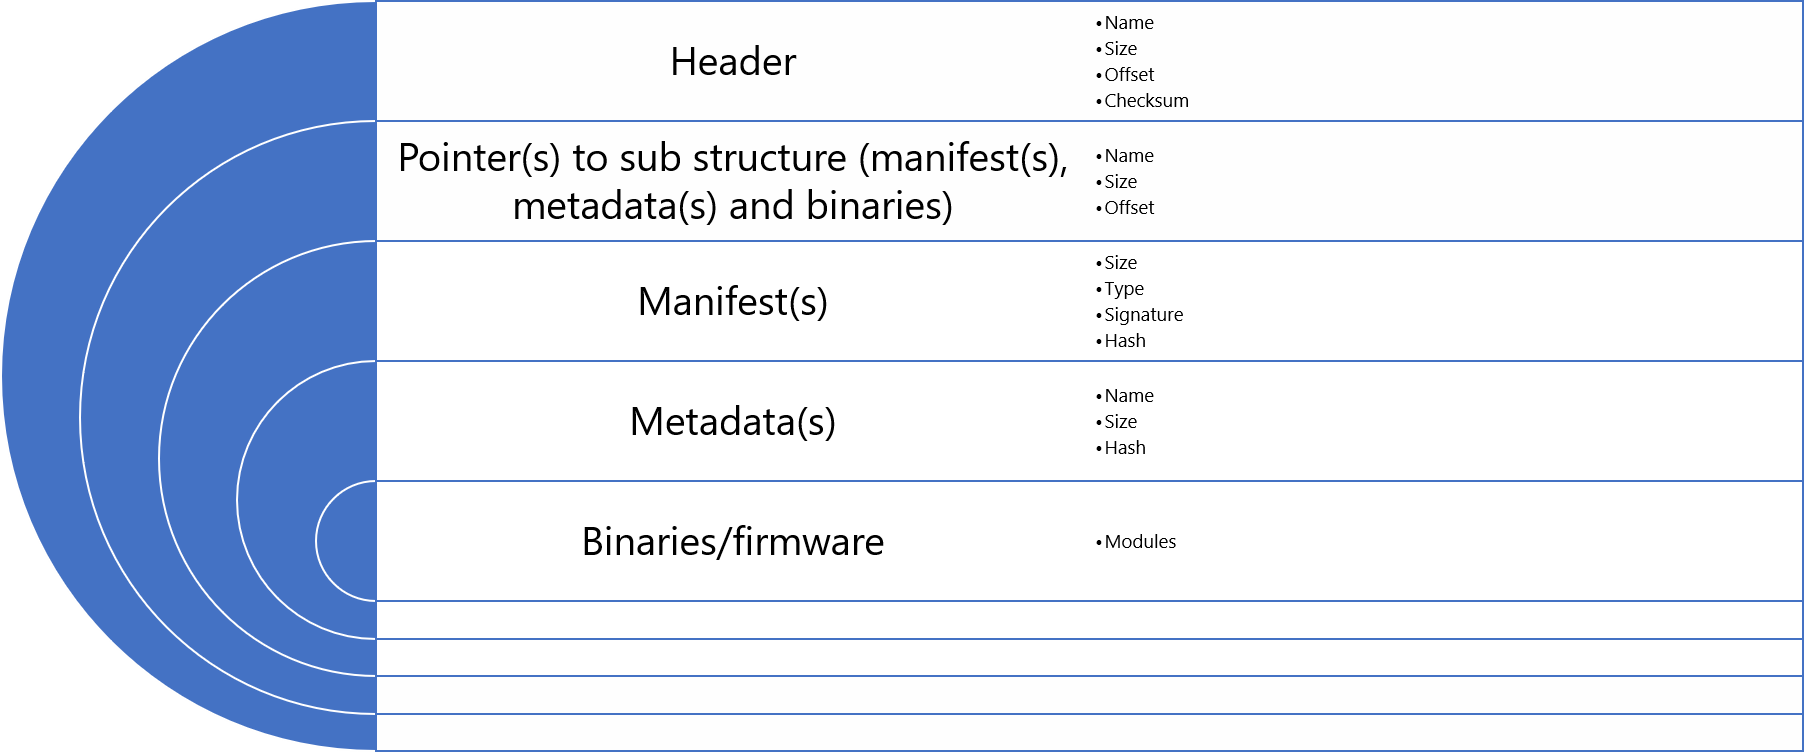
\includegraphics[width=0.9\linewidth]{Im/figures/proposed-work/proposed-structure-firmware-signing}
        \caption{Proposed Structure for firmware signing}\label{fig:proposed-work-proposed-structure-firmware-signing}
    \end{figure}
\end{frame}


\begin{frame}{IP firmware Integration: Outcome}
    \begin{itemize}
        \item Removal of IP dependency during firmware loading
        \item IP Subsystem :
        \begin{itemize}
            \item Loader and Verifier
            \item IP is always consumer
        \end{itemize}
        \item Signature verification using SHA hash algorithm
        \item Seamless Integration of any other hash algorithm for verification
        \item Hardware based and Software based verification support
        \item Prevent common security threats
        \item Allow easier OEM adoption and modification based on the respective design
        \item Reusability/Portability of design across many IPs
        \item Generic design which supports any new IP integration
    \end{itemize}
\end{frame}